% SPDX-License-Identifier: CC-BY-SA-4.0
%
% Copyright (c) 2020 Philipp Le
%
% Except where otherwise noted, this work is licensed under a
% Creative Commons Attribution-ShareAlike 4.0 License.
%
% Please find the full copy of the licence at:
% https://creativecommons.org/licenses/by-sa/4.0/legalcode

\phantomsection
\addcontentsline{toc}{section}{Exercise 5}
\section*{Exercise 5}

%%%%%%%%%%%%%%%%%%%%%%%%%%%%%%%%%%%%%%%%%%%%%%%%%%%%%%%%%%%%%%%%%%%%%%%%%%%%%%%
\begin{question}[subtitle={Mixers}]
	\begin{tasks}
		\task
		Is the mixer a linear device like filters and amplifiers?
		\task
		What is the difference between unbalanced and balanced mixers?
		\task
		Why do mixers need a non-linear component?
	\end{tasks}
\end{question}

\begin{solution}
	\begin{tasks}
		\task
		No, it is non-linear. Its non-linear component is responsible for the mixing.
		
		A linear device would fulfil:
		\begin{equation*}
			M\left(a x + b y\right) = a M(x) + b M(y)
		\end{equation*}
		where $M(x)$ is the characteristic curve of the device. Especially the frequencies would be retained. A mixer changes the frequencies.
		
		\task
		\begin{itemize}
			\item At least one input of a balanced mixer is balanced (differential). It is capable of suppressing the carrier.
			\item An unbalanced mixer has only unbalanced (single-ended) inputs. The carrier is not suppressed.
		\end{itemize}
	
		\task
		The non-linear component is responsible for the mixing process.
		
		The characteristic curve of the non-linearity can be decomposed using a Taylor series:
		\begin{equation*}
			\begin{split}
				x_{o} &= M(x_{i} + x_{LO} + a) = \sum\limits_{n=0}^{\infty} \frac{1}{n!} \left.\frac{\mathrm{d}^n M(x)}{\mathrm{d} x^n}\right|_{x=a} \left(x_{i} + x_{LO} + a - a\right)^n \\
				 &= M(a) + \underbrace{M^{(1)}(a) \left(x_{i} + x_{LO}\right)}_{\text{Linear term}} + \underbrace{\frac{M^{(2)}(a)}{2} \left(x_{i} + x_{LO}\right)^2}_{\text{Quadratic term}} + \underbrace{\frac{M^{(3)}(a)}{6} \left(x_{i} + x_{LO}\right)^3}_{\text{Qubic term}} + \dots
				\end{split}
		\end{equation*}
		
		The quadratic term is the important part in the mixing process.
		\begin{equation*}
			\left(x_{i} + x_{LO}\right)^2 = x_{i}^2 + 2 \underbrace{x_{i} x_{LO}}_{\text{Mixing}} + x_{LO}^2
		\end{equation*}
		
		The multiplication in the time-domain becomes a convolution in the frequency-domain, which represents the mixing process.
	\end{tasks}
\end{solution}

%%%%%%%%%%%%%%%%%%%%%%%%%%%%%%%%%%%%%%%%%%%%%%%%%%%%%%%%%%%%%%%%%%%%%%%%%%%%%%%
\begin{question}[subtitle={Mirror frequencies}]
	This is simplified block diagram of a receiver with two analogue mixing stages (super-heterodyne). The bandpass has a centre frequency of \SI{481}{MHz}.
	\begin{figure}[H]
		\centering
		\begin{adjustbox}{scale=0.8}
			\begin{circuitikz}
				\node[mixer](Mixer1){};
				\node[oscillator, below=1cm of Mixer1](LO){};
				\node[mixer, right=1.5cm of Mixer1](Mixer2){};
				\node[oscillator, below=1cm of Mixer2](BFO){};
				\node[adcshape, right=2cm of Mixer2](ADC){};
				\node[block, draw, right=1cm of ADC](Baseband){Digital signal\\ processing};
				
				\draw (LO.south) node[below,align=center,yshift=-5mm]{LO};
				\draw (BFO.south) node[below,align=center,yshift=-5mm]{Fixed\\ \SI{480}{MHz}};
				\draw (Mixer1.north) node[above,align=center,yshift=3mm]{1st Mixer};
				\draw (Mixer2.north) node[above,align=center,yshift=3mm]{2nd Mixer};
				
				\draw (Mixer1.west) -- ++(-1cm,0) node[rxantenna,xscale=-1]{};
				
				\draw[-latex] (LO.north) -- (Mixer1.south);
				\draw[-latex] (BFO.north) -- (Mixer2.south);
				\draw[-latex] (Mixer1.east) to[bandpass] node[midway,align=center,yshift=-8mm,xshift=-6mm]{\SI{481}{MHz}} (Mixer2.west);
				\draw[-latex] (Mixer2.east) to[lowpass] (ADC.west);
				\draw[-latex] (ADC.east) -- (Baseband.west);
			\end{circuitikz}
		\end{adjustbox}
	\end{figure}
	A signal of \SI{868}{MHz} should be received. The baseband is not zero-IF. The signal shall be mixed down to \SI{1}{MHz} centre frequency, so that the signal can be processed digitally.

	\begin{tasks}
		\task
		How much is the minimum ADC sampling rate?
		\task
		To which frequencies can the LO be tuned to?
		\task
		The electromagnetic spectrum is shared with lots of other users. Which important piece is missing in the receiver signal chain?
		%\task
		%An IQ demodulator is used instead of the single mixer. Sketch the spectrum of the complex-valued baseband signal for both possible LO frequencies!
	\end{tasks}
\end{question}

\begin{solution}
	\begin{tasks}
		\task
		According to the Shannon-Nyquist theorem, minimum \SI{2}{MHz}.
		
		\begin{remark}
			A signal is practically never mixed to exactly \SI{0}{Hz}. All ADC have a DC bias. The sampled signal is superimposed by a DC voltage at \SI{0}{Hz} in the time-domain. This adds an error. Therefore, the signal shifted some \si{kHz} away from DC.
		\end{remark}
		
		\task
		The bandpass has a centre frequency of \SI{481}{MHz}. Therefore, \SI{481}{MHz} is the desired output of mixing stage one.
		
		
		Either
		\begin{itemize}
			\item $\SI{868}{MHz} - \SI{481}{MHz} = \SI{387}{MHz}$ or
			\item $\SI{868}{MHz} + \SI{481}{MHz} = \SI{1349}{MHz}$
		\end{itemize}
		will work.
		
		The first frequency of \SI{387}{MHz} is clear. If the two inputs \SI{387}{MHz} (LO) and \SI{868}{MHz} (RF) are applied, the two outputs are $\SI{868}{MHz} - \SI{387}{MHz} = \SI{481}{MHz}$ and $\SI{868}{MHz} + \SI{387}{MHz} = \SI{1255}{MHz}$. The second output is rejected by the bandpass filter.
		
		The second frequency of \SI{1349}{MHz} needs further explanation. If the two inputs \SI{1349}{MHz} (LO) and \SI{868}{MHz} (RF) are applied, the two outputs are $\SI{1349}{MHz} - \SI{868}{MHz} = \SI{481}{MHz}$ and $\SI{1349}{MHz} + \SI{868}{MHz} = \SI{2217}{MHz}$. The second output is rejected by the bandpass filter.
		
		\begin{remark}
			The super-heterodyne receiver has two mixer stages. The first mixer defines the RF frequency which should be received. The first intermediate frequency is fixed. The bandpass filter has a high frequency, so that it is super-selective and neighbouring users are eliminated and cannot disturb the wanted signal.
		\end{remark}
		
		\task
		The receiver receives on mirror frequencies.
		\begin{itemize}
			\item $\SI{481}{MHz} - \SI{387}{MHz} = \SI{94}{MHz}$ (for $f_{LO} = \SI{387}{MHz}$) or
			\item $\SI{1349}{MHz} + \SI{481}{MHz} = \SI{1830}{MHz}$ (for $f_{LO} = \SI{1349}{MHz}$)
		\end{itemize}
		will be received, too. The signals that these RF frequencies will superimpose the signal mixed down from the desired signal at \SI{868}{MHz}.
		
		The input of the first mixer must be filtered by either
		\begin{itemize}
			\item a lowpass (only for $f_{LO} = \SI{1349}{MHz}$ to block the mirror frequency at \SI{1828}{MHz}),
			\item a highpass (only for $f_{LO} = \SI{387}{MHz}$ to block the mirror frequency at \SI{92}{MHz}) or
			\item a bandpass (works for both LO configurations).
		\end{itemize}
	\end{tasks}
\end{solution}

%%%%%%%%%%%%%%%%%%%%%%%%%%%%%%%%%%%%%%%%%%%%%%%%%%%%%%%%%%%%%%%%%%%%%%%%%%%%%%%
\begin{question}[subtitle={Constellation diagrams}]
	Draw a constellation diagram of:
	\begin{tasks}
		\task
		ASK (with 2 steps)
		\task
		BPSK
		\task
		QPSK
		\task
		16-QAM
	\end{tasks}
\end{question}

\begin{solution}
	\begin{tasks}
		\task
		\begin{figure}[H]
			\centering
			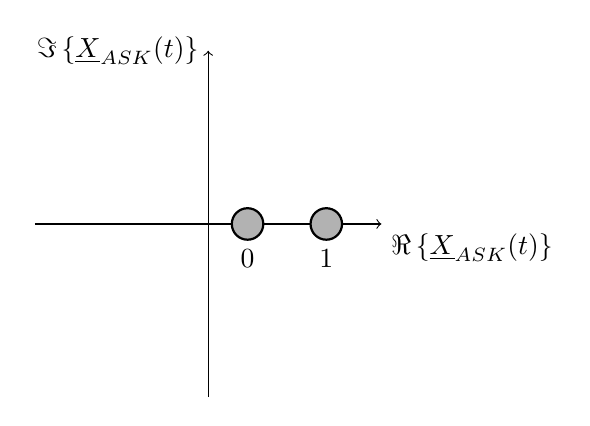
\begin{tikzpicture}
				\draw[->] (-2.2,0) -- (2.2,0) node[below right, align=left]{$\Re\left\{\underline{X}_{ASK}(t)\right\}$};
				\draw[->] (0,-2.2) -- (0,2.2) node[left, align=right]{$\Im\left\{\underline{X}_{ASK}(t)\right\}$};
				
				\draw[black,thick,fill=gray!60] (0:0.5) ++(0,-0.2) arc(-90:270:0.2) node[below,align=center]{0};
				\draw[black,thick,fill=gray!60] (0:1.5) ++(0,-0.2) arc(-90:270:0.2) node[below,align=center]{1};
			\end{tikzpicture}
		\end{figure}
		
		\task
		\begin{figure}[H]
			\centering
			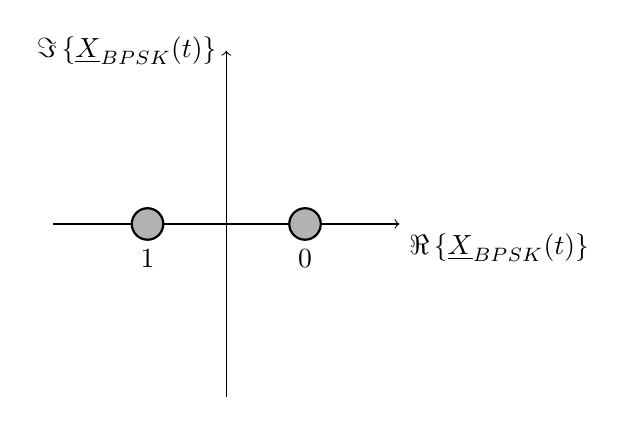
\begin{tikzpicture}
				\draw[->] (-2.2,0) -- (2.2,0) node[below right, align=left]{$\Re\left\{\underline{X}_{BPSK}(t)\right\}$};
				\draw[->] (0,-2.2) -- (0,2.2) node[left, align=right]{$\Im\left\{\underline{X}_{BPSK}(t)\right\}$};
				
				\draw[black,thick,fill=gray!60] (0:1) ++(0,-0.2) arc(-90:270:0.2) node[below,align=center]{0};
				\draw[black,thick,fill=gray!60] (180:1) ++(0,-0.2) arc(-90:270:0.2) node[below,align=center]{1};
			\end{tikzpicture}
		\end{figure}
		
		\task
		\begin{figure}[H]
			\centering
			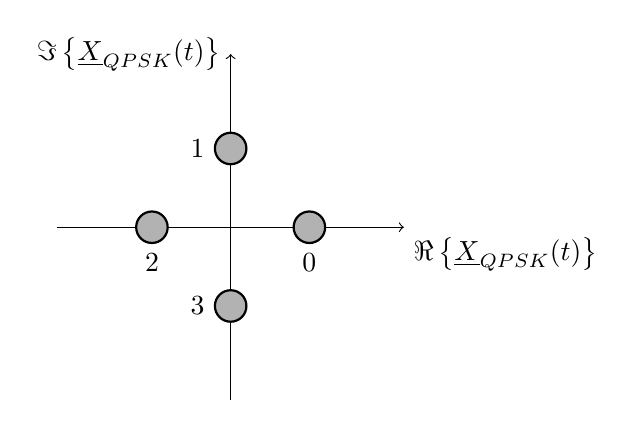
\begin{tikzpicture}
				\draw[->] (-2.2,0) -- (2.2,0) node[below right, align=left]{$\Re\left\{\underline{X}_{QPSK}(t)\right\}$};
				\draw[->] (0,-2.2) -- (0,2.2) node[left, align=right]{$\Im\left\{\underline{X}_{QPSK}(t)\right\}$};
				
				\draw[black,thick,fill=gray!60] (0:1) ++(0,-0.2) arc(-90:270:0.2) node[below,align=center]{0};
				\draw[black,thick,fill=gray!60] (90:1) ++(-0.2,0) arc(-180:180:0.2) node[left,align=right]{1};
				\draw[black,thick,fill=gray!60] (180:1) ++(0,-0.2) arc(-90:270:0.2) node[below,align=center]{2};
				\draw[black,thick,fill=gray!60] (270:1) ++(-0.2,0) arc(-180:180:0.2) node[left,align=right]{3};
			\end{tikzpicture}
		\end{figure}
		
		\task
		\begin{figure}[H]
			\centering
			\begin{adjustbox}{scale=1}
				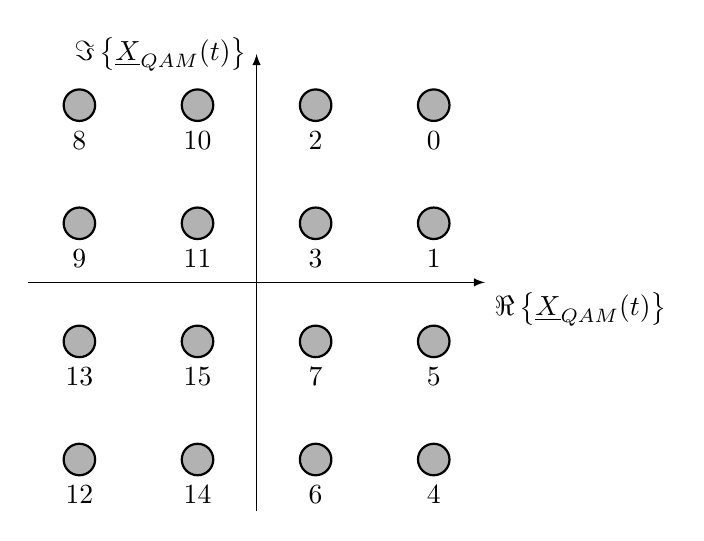
\begin{tikzpicture}[scale=1]
				\draw[-latex] (-2.9,0) -- (2.9,0) node[below right, align=left]{$\Re\left\{\underline{X}_{QAM}(t)\right\}$};
				\draw[-latex] (0,-2.9) -- (0,2.9) node[left, align=right]{$\Im\left\{\underline{X}_{QAM}(t)\right\}$};
				
				\draw[black,thick,fill=gray!60] (2.25,2.25) ++(0,-0.2) arc(-90:270:0.2) node[below,align=center]{0};
				\draw[black,thick,fill=gray!60] (2.25,0.75) ++(0,-0.2) arc(-90:270:0.2) node[below,align=center]{1};
				\draw[black,thick,fill=gray!60] (0.75,2.25) ++(0,-0.2) arc(-90:270:0.2) node[below,align=center]{2};
				\draw[black,thick,fill=gray!60] (0.75,0.75) ++(0,-0.2) arc(-90:270:0.2) node[below,align=center]{3};
				
				\draw[black,thick,fill=gray!60] (2.25,-2.25) ++(0,-0.2) arc(-90:270:0.2) node[below,align=center]{4};
				\draw[black,thick,fill=gray!60] (2.25,-0.75) ++(0,-0.2) arc(-90:270:0.2) node[below,align=center]{5};
				\draw[black,thick,fill=gray!60] (0.75,-2.25) ++(0,-0.2) arc(-90:270:0.2) node[below,align=center]{6};
				\draw[black,thick,fill=gray!60] (0.75,-0.75) ++(0,-0.2) arc(-90:270:0.2) node[below,align=center]{7};
				
				\draw[black,thick,fill=gray!60] (-2.25,2.25) ++(0,-0.2) arc(-90:270:0.2) node[below,align=center]{8};
				\draw[black,thick,fill=gray!60] (-2.25,0.75) ++(0,-0.2) arc(-90:270:0.2) node[below,align=center]{9};
				\draw[black,thick,fill=gray!60] (-0.75,2.25) ++(0,-0.2) arc(-90:270:0.2) node[below,align=center]{10};
				\draw[black,thick,fill=gray!60] (-0.75,0.75) ++(0,-0.2) arc(-90:270:0.2) node[below,align=center]{11};
				
				\draw[black,thick,fill=gray!60] (-2.25,-2.25) ++(0,-0.2) arc(-90:270:0.2) node[below,align=center]{12};
				\draw[black,thick,fill=gray!60] (-2.25,-0.75) ++(0,-0.2) arc(-90:270:0.2) node[below,align=center]{13};
				\draw[black,thick,fill=gray!60] (-0.75,-2.25) ++(0,-0.2) arc(-90:270:0.2) node[below,align=center]{14};
				\draw[black,thick,fill=gray!60] (-0.75,-0.75) ++(0,-0.2) arc(-90:270:0.2) node[below,align=center]{15};
				\end{tikzpicture}
			\end{adjustbox}
		\end{figure}
	\end{tasks}
\end{solution}

%%%%%%%%%%%%%%%%%%%%%%%%%%%%%%%%%%%%%%%%%%%%%%%%%%%%%%%%%%%%%%%%%%%%%%%%%%%%%%%
\begin{question}[subtitle={Constellation diagrams}]
	A QPSK modulator has the following mapping and symbol constellation:
	\begin{table}[H]
		\centering
		\begin{tabular}{|l|l|l|}
			\hline
			Data & Symbol & Phasor \\
			\hline
			\hline
			$(00)_2$ & 0 & $\SI{2}{mV} \cdot e^{j 0}$ \\
			\hline
			$(01)_2$ & 1 & $\SI{2}{mV} \cdot e^{j \frac{\pi}{2}}$ \\
			\hline
			$(10)_2$ & 2 & $\SI{2}{mV} \cdot e^{j \pi}$ \\
			\hline
			$(11)_2$ & 3 & $\SI{2}{mV} \cdot e^{j \frac{3 \pi}{2}}$ \\
			\hline
		\end{tabular}
	\end{table}
	The carrier is:
	\begin{equation*}
		x_C(t) = \SI{2}{mV} \cdot \cos\left(2\pi \cdot \SI{50}{MHz} \cdot t\right)
	\end{equation*}
	The symbol rate is $\SI{25}{MHz}$. After the DAC, an low-pass filter with $\SI{25}{MHz}$ cut-off frequency is applied.
	
	\begin{tasks}
		\task
		How much is the transmission bandwidth (narrowband case)?
		\task
		How many bits can be encoded per QPSK symbol? How many symbols are required to encode one byte (8 bits)?
		\task
		Draw the constellation diagram!
		\task
		The data byte $(2D)_{16}$ shall be transmitted. Give the sequence of phasors representing the data byte!
		\task
		Explain the problem with inter-symbol interference! Describe a solution!
		\task
		Plot the I and Q baseband signals! Plot the RF signal after IQ modulation! The baseband filter shall be neglected; consider ideal symbols.
		\task
		The following phasors are received at the receiver:
		\begin{equation*}
			\left[\SI{1.5}{mV} \cdot e^{j \SI{120}{\degree}}, \SI{1.5}{mV} \cdot e^{j \SI{300}{\degree}}, \SI{1.5}{mV} \cdot e^{j \SI{30}{\degree}}, \SI{1.5}{mV} \cdot e^{j \SI{210}{\degree}}\right]
		\end{equation*}
		What would the decoded data be? What is the matter?
	\end{tasks}
\end{question}

\begin{solution}
	\begin{tasks}
		\task
		Due to the applied lowpass filter, the bandwidth of the signal after the DAC is $\SI{25}{MHz}$. The transmission bandwidth of the QPSK is that of the PM. Here the narrowband PM is considered, so that the transmission bandwidth is $\SI{25}{MHz}$.
		
		\task
		One symbol has $K_m = 4$ states. It can encode \SI{2}{bit}.
		\begin{equation*}
			B = \log_2 K_m = 2
		\end{equation*}
		
		Consequently, if the data is \SI{8}{bit}, 4 symbols are required.
		
		\task
		\begin{figure}[H]
			\centering
			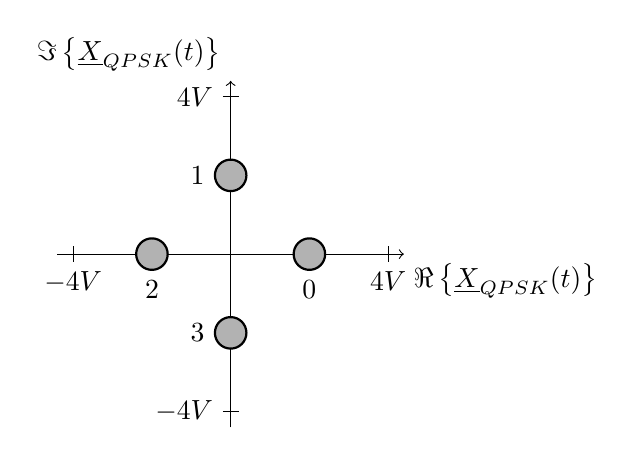
\begin{tikzpicture}
				\draw[->] (-2.2,0) -- (2.2,0) node[below right, align=left]{$\Re\left\{\underline{X}_{QPSK}(t)\right\}$};
				\draw[->] (0,-2.2) -- (0,2.2) node[above left, align=right]{$\Im\left\{\underline{X}_{QPSK}(t)\right\}$};
				
				\draw (2,-0.1) node[below]{$\SI{4}{V}$} -- (2,0.1);
				\draw (-2,-0.1) node[below]{$-\SI{4}{V}$} -- (-2,0.1);
				\draw (-0.1,2) node[left]{$\SI{4}{V}$} -- (0.1,2);
				\draw (-0.1,-2) node[left]{$-\SI{4}{V}$} -- (0.1,-2);
				
				\draw[black,thick,fill=gray!60] (0:1) ++(0,-0.2) arc(-90:270:0.2) node[below,align=center]{0};
				\draw[black,thick,fill=gray!60] (90:1) ++(-0.2,0) arc(-180:180:0.2) node[left,align=right]{1};
				\draw[black,thick,fill=gray!60] (180:1) ++(0,-0.2) arc(-90:270:0.2) node[below,align=center]{2};
				\draw[black,thick,fill=gray!60] (270:1) ++(-0.2,0) arc(-180:180:0.2) node[left,align=right]{3};
			\end{tikzpicture}
		\end{figure}
		
		\task
		The hexadecimal value $(2D)_{16} = (00101101)_{2}$ in binary notation.
		
		Using the encoding:
		\begin{table}[H]
			\centering
			\begin{tabular}{|l|l|l|}
				\hline
				Data part & Symbol & Phasor \\
				\hline
				\hline
				$(00)_2$ & 0 & $\SI{2}{mV} \cdot e^{j 0}$ \\
				\hline
				$(10)_2$ & 2 & $\SI{2}{mV} \cdot e^{j \pi}$ \\
				\hline
				$(11)_2$ & 3 & $\SI{2}{mV} \cdot e^{j \frac{3 \pi}{2}}$ \\
				\hline
				$(01)_2$ & 1 & $\SI{2}{mV} \cdot e^{j \frac{\pi}{2}}$ \\
				\hline
			\end{tabular}
		\end{table}
	
		The series of phasors is:
		\begin{equation*}
			\left[\SI{2}{mV} \cdot e^{j \SI{0}{\degree}}, \SI{2}{mV} \cdot e^{j \SI{180}{\degree}}, \SI{2}{mV} \cdot e^{j \SI{270}{\degree}}, \SI{2}{mV} \cdot e^{j \SI{90}{\degree}}\right]
		\end{equation*}
		or in radians
		\begin{equation*}
			\left[\SI{2}{mV} \cdot e^{j \SI{0}{\degree}}, \SI{2}{mV} \cdot e^{j \pi}, \SI{2}{mV} \cdot e^{j \frac{3 \pi}{2}}, \SI{2}{mV} \cdot e^{j \frac{\pi}{2}}\right]
		\end{equation*}
		
		\task
		\begin{itemize}
%			\item The baseband signal is band-limited by an ideal low-pass filter.
%			\item An ideal low-pass filter has a rectangular shape in the frequency-domain.
%			\item The inverse Fourier transform of the rectangular shape is a sinc-function in the time-domain.
%			\item The ideal low-pass filter's impulse response is a sinc-function.
%			\item The series of symbols is now convoluted with the sinc-function (impulse response of the filter).
%			\item The ideal symbols, which are a rectangular function, are flattened. Their edges are rounded and spread across the time axis.
			\item The baseband signal is band-limited by an low-pass filter.
			\item Let's consider an ideal filter:
			\begin{itemize}
				\item An ideal low-pass filter has a rectangular shape in the frequency-domain.
				\item The inverse Fourier transform of the rectangular shape is a sinc-function in the time-domain.
				\item The ideal low-pass filter's impulse response is a sinc-function.
			\end{itemize}
			\item \begin{remark}The impulse response of a real low-pass filter is of course not exactly the sinc-function, but some kind of exponential function.\end{remark}
			\item The series of symbols is now convoluted with the impulse response of the filter.
			\item The ideal symbols, which are a rectangular function, are flattened. Their edges are rounded and spread across the time axis.
		\end{itemize}
		The flattened symbols will interfere with their neighbouring symbols. The decoding may fail. The data error probability is increased.
		
		\begin{figure}[H]
			\centering
			\begin{tikzpicture}
				\begin{axis}[
					height={0.15\textheight},
					width=0.7\linewidth,
					scale only axis,
					xlabel={$t$},
					ylabel={$x_{sym}(t)$},
					%grid style={line width=.6pt, color=lightgray},
					%grid=both,
					grid=none,
					legend pos=outer north east,
					axis y line=middle,
					axis x line=middle,
					every axis x label/.style={
						at={(ticklabel* cs:1.05)},
						anchor=north,
					},
					every axis y label/.style={
						at={(ticklabel* cs:1.05)},
						anchor=east,
					},
					xmin=-0.5,
					xmax=8.5,
					ymin=0,
					ymax=1.7,
					%xtick={0,0.125,...,1},
					%xticklabels={$- \omega_S$, $- \frac{\omega_S}{2}$, $0$, $\frac{\omega_S}{2}$, $\omega_S$},
					%ytick={0},
				]
					\addplot[blue,smooth] coordinates {(-1.5,0) (0,0.5) (0.5,0.85) (1,1) (1.5,0.85) (2,0.5) (3.5,0)};
					\addplot[red,smooth] coordinates {(0.5,0) (2,0.5) (2.5,0.85) (3,1) (3.5,0.85) (4,0.5) (5.5,0)};
					\addplot[green,smooth] coordinates {(2.5,0) (4,0.5) (4.5,0.85) (5,1) (5.5,0.85) (6,0.5) (7.5,0)};
					\addplot[olive,smooth] coordinates {(4.5,0) (6,0.5) (6.5,0.85) (7,1) (7.5,0.85) (8,0.5) (9.5,0)};
					
					\draw[dashed] (axis cs:2,0) -- (axis cs:2,1.2);
					\draw[dashed] (axis cs:4,0) -- (axis cs:4,1.2);
					\draw[latex-latex] (axis cs:2,1.1) -- node[midway,above,align=center]{Symbol period $T_{sym}$} (axis cs:4,1.1);
				\end{axis}
			\end{tikzpicture}
		\end{figure}
	
		A guard interval must be inserted after each symbol to reduce the inter-symbol interference.
		\begin{itemize}
			\item The guard interval must be long enough so that the contribution of one signal to its neighbours is so weak, that the symbol detection works with a low data error probability.
			\item The guard interval will reduce the effective symbol rate whilst keeping the transmission bandwidth of the signal constant.
			\item Keeping the effective symbol rate by reducing the symbol width $T_w$ (to make space for the guard interval) is also possible. But this comes a t the drawback of increasing the transmission bandwidth, which would be $1/T_w$. This is not always possible because the bandwidth is restricted by technical norms or laws.
		\end{itemize}
		
		\task
		I component:
		\begin{figure}[H]
			\centering
			\begin{tikzpicture}
				\begin{axis}[
					height={0.1\textheight},
					width=0.6\linewidth,
					scale only axis,
					xlabel={$t$ in \si{ns}},
					ylabel={$\Re\left\{\underline{x}_B(t)\right\}$},
					%grid style={line width=.6pt, color=lightgray},
					%grid=both,
					grid=none,
					legend pos=outer north east,
					axis y line=middle,
					axis x line=middle,
					every axis x label/.style={
						at={(ticklabel* cs:1.05)},
						anchor=north,
					},
					every axis y label/.style={
						at={(ticklabel* cs:1.05)},
						anchor=east,
					},
					xmin=-0.5,
					xmax=8.5,
					ymin=-1.2,
					ymax=1.2,
					xtick={0,2,4,6,8},
					xticklabels={0, 40, 80, 120, 160},
					%ytick={0},
				]
					\addplot[red] coordinates {(0,1) (2,1)};
					\addplot[red] coordinates {(2,-1) (4,-1)};
					\addplot[red] coordinates {(4,0) (8,0)};
					
					\draw[dashed] (axis cs:2,-1.6) -- (axis cs:2,1.2);
					\draw[dashed] (axis cs:4,-1.6) -- (axis cs:4,1.2);
					\draw[dashed] (axis cs:6,-1.6) -- (axis cs:6,1.2);
					\draw[dashed] (axis cs:8,-1.6) -- (axis cs:8,1.2);
					
					\draw (1,-1.5) node{0};
					\draw (3,-1.5) node{2};
					\draw (5,-1.5) node{3};
					\draw (7,-1.5) node{1};
				\end{axis}
			\end{tikzpicture}
		\end{figure}
	
		Q component:
		\begin{figure}[H]
			\centering
			\begin{tikzpicture}
				\begin{axis}[
					height={0.1\textheight},
					width=0.6\linewidth,
					scale only axis,
					xlabel={$t$ in \si{ns}},
					ylabel={$\Im\left\{\underline{x}_B(t)\right\}$},
					%grid style={line width=.6pt, color=lightgray},
					%grid=both,
					grid=none,
					legend pos=outer north east,
					axis y line=middle,
					axis x line=middle,
					every axis x label/.style={
						at={(ticklabel* cs:1.05)},
						anchor=north,
					},
					every axis y label/.style={
						at={(ticklabel* cs:1.05)},
						anchor=east,
					},
					xmin=-0.5,
					xmax=8.5,
					ymin=-1.2,
					ymax=1.2,
					xtick={0,2,4,6,8},
					xticklabels={0, 40, 80, 120, 160},
					%ytick={0},
				]
					\addplot[red] coordinates {(0,0) (4,0)};
					\addplot[red] coordinates {(4,-1) (6,-1)};
					\addplot[red] coordinates {(6,1) (8,1)};
					
					\draw[dashed] (axis cs:2,-1.6) -- (axis cs:2,1.2);
					\draw[dashed] (axis cs:4,-1.6) -- (axis cs:4,1.2);
					\draw[dashed] (axis cs:6,-1.6) -- (axis cs:6,1.2);
					\draw[dashed] (axis cs:8,-1.6) -- (axis cs:8,1.2);
					
					\draw (1,-1.5) node{0};
					\draw (3,-1.5) node{2};
					\draw (5,-1.5) node{3};
					\draw (7,-1.5) node{1};
				\end{axis}
			\end{tikzpicture}
		\end{figure}
	
		RF signal after IQ modulation:
		\begin{figure}[H]
			\centering
			\begin{tikzpicture}
				\begin{axis}[
					height={0.1\textheight},
					width=0.6\linewidth,
					scale only axis,
					xlabel={$t$ in \si{ns}},
					ylabel={$u_{RF}(t)$ in \si{mV}},
					%grid style={line width=.6pt, color=lightgray},
					%grid=both,
					grid=none,
					legend pos=outer north east,
					axis y line=middle,
					axis x line=middle,
					every axis x label/.style={
						at={(ticklabel* cs:1.05)},
						anchor=north,
					},
					every axis y label/.style={
						at={(ticklabel* cs:1.05)},
						anchor=east,
					},
					xmin=-0.5,
					xmax=8.5,
					ymin=-2.2,
					ymax=2.2,
					xtick={0,2,4,6,8},
					xticklabels={0, 40, 80, 120, 160},
					%ytick={0},
				]
					
					\addplot[red, smooth, domain=0:2, samples=50] plot(\x, {2*cos(deg(2*pi*1*\x))});
					\addplot[red, smooth, domain=2:4, samples=50] plot(\x, {2*cos(deg(2*pi*1*\x)+180)});
					\addplot[red, smooth, domain=4:6, samples=50] plot(\x, {2*cos(deg(2*pi*1*\x)+270)});
					\addplot[red, smooth, domain=6:8, samples=50] plot(\x, {2*cos(deg(2*pi*1*\x)+90)});
					
					\draw[dashed] (axis cs:2,-1.6) -- (axis cs:2,1.2);
					\draw[dashed] (axis cs:4,-1.6) -- (axis cs:4,1.2);
					\draw[dashed] (axis cs:6,-1.6) -- (axis cs:6,1.2);
					\draw[dashed] (axis cs:8,-1.6) -- (axis cs:8,1.2);
					
					\draw (1,-1.5) node{0};
					\draw (3,-1.5) node{2};
					\draw (5,-1.5) node{3};
					\draw (7,-1.5) node{1};
				\end{axis}
			\end{tikzpicture}
		\end{figure}
		
		\task
		Given that the decoder decides to assign the received phasor to the closest symbol, the data would be: $(01)_2 (11)_2 (00)_2 (10)_2$ or as a byte $(10001101)_2$ (the firstly received symbol is aligned to the right).
	\end{tasks}
\end{solution}

%%%%%%%%%%%%%%%%%%%%%%%%%%%%%%%%%%%%%%%%%%%%%%%%%%%%%%%%%%%%%%%%%%%%%%%%%%%%%%%
%\begin{question}[subtitle={Decibel}]
%	\begin{tasks}
%	\end{tasks}
%\end{question}
%
%\begin{solution}
%	\begin{tasks}
%	\end{tasks}
%\end{solution}
